\documentclass[final, english, english, a4paper, 12pt, numbers=noenddot, % Bei Änderung der Sprache 2 x kompilieren!
% tudscr spezifische Einstellungen
cd=false,
cdfont=false,cdfont=nohead,
cdmath=false,
cdhead=false,
cdfoot=true,
cdcover=monochrome,
cdgeometry=asymmetric,
declaration=heading,
declaration=notoc,
abstract=heading,
]{tudscrreprt}

%################ Hilfreiche Pakete laden #######################

%################ Hilfreiche Pakete laden #######################

\usepackage{settings/tudbwlimPackages}
\usepackage{settings/tudbwlimStyle}
\usepackage{scrhack}
\usepackage{microtype}
\usepackage{tikz,pgfplots}
\pgfplotsset{compat=newest}
\usepackage[chapter]{algorithm} % Falls das Paket floatrow geladen wird, muss dieses Paket danach geladen werden.
\iflanguage{english}{\floatname{algorithm}{Algorithm}\renewcommand{\listalgorithmname}{List of Algorithms}}{\floatname{algorithm}{Algorithmus}\renewcommand{\listalgorithmname}{Algorithmenverzeichnis}} % Algorithm-Umgebung an die verwendete Sprache anpassen
\usepackage{comment}
\usepackage{subcaption}
\usepackage{caption}
\usetikzlibrary{positioning}
\usetikzlibrary{mindmap}
\usepackage{graphicx}
\usepackage{float}
\usepackage{longtable}
\usepackage{xparse} % for \NewDocumentCommand
\usepackage{multirow}
\usepackage{array}
\usepackage{makecell}
\usepackage[justification=centering]{caption} % Für die Zentrierung der Bildunterschrift

%################ Notwendige Pakete laden #######################


\usepackage[bibencoding=auto,citestyle=authoryear-ibid,bibstyle=authoryear,maxcitenames=3,maxbibnames=10, backend = biber]{biblatex}% Vergessen Sie nicht in den Optionen das Bibliographieprogramm auf "biber" umzustellen! Um die Vorlage mit BibTeX nutzen zu können, muss die Option "backend=bibtex" übergeben werden. Es ist jedoch biber zu empfehlen, beachten Sie dazu die Hinweise der biblatex-Paketdokumentation im Abschnitt 3.15 "Using the fallback BibtTeX backend".
\usepackage{settings/BiblatexSetup}

\AfterPackage*{biblatex}%
{
    \RequirePackage[breaklinks=true, colorlinks=true, linktoc=section, linkcolor=blue, citecolor=black, hidelinks]{hyperref}
    % Da hyperref allerhand Veränderungen an vielen Standardbefehlen vornimmt, sollte dieses als letztes in der Präambel eingebunden werden. Nur Pakete, bei denen in der Dokumentation explizit darauf hingewiesen wird, dass diese nach hyperref zu laden sind, sollten auch danach folgen.
    \hypersetup{pdfprintscaling=None} % gleiches Verhalten, auch ohne hyperref, liefert: \pdfcatalog{/ViewerPreferences<</PrintScaling/None>>}
    \usepackage{footnote} % https://tex.stackexchange.com/questions/207192/footcite-in-float-caption
    \makesavenoteenv{figure}
    \makesavenoteenv{table}
    \makesavenoteenv{algorithm}
}


\AfterPackage*{hyperref}
{
    \RequirePackage[automake,acronym,symbols,nomain,translate=babel]{glossaries}
    \usepackage{settings/GlossariesSetup}
}
%############## Own commands #####################´
\newcommand{\parbreak}{\vspace{\baselineskip}\noindent}
\newcommand{\gendreauDataSet}{Gendreau (2006)}
\newcommand{\mouraDataSet}{Moura (2009)}
\newcommand{\ceschiaDataSet}{Ceschia (2013)}
\newcommand{\krebsADataSet}{Krebs (2021a)}
\newcommand{\krebsBDataSet}{Krebs (2021b)}
\newcommand{\gendreauDataSetText}{\gendreauDataSet\ }
\newcommand{\mouraDataSetText}{\mouraDataSet\ }
\newcommand{\ceschiaDataSetText}{\ceschiaDataSet\ }
\newcommand{\krebsADataSetText}{\krebsADataSet\ }
\newcommand{\krebsBDataSetText}{\krebsBDataSet\ }

%############## Ideas for packages #####################´
% Folgende auskommentierte Pakete sind als Vorschläge zu verstehen. Für Funktionsweise und Anwendungsfälle wird auf das Benutzerhandbuch "tudscr.pdf" (http://mirrors.ctan.org/macros/latex/contrib/tudscr/doc/tudscr.pdf) oder auf die entsprechende CTAN Dokumentation verwiesen.
%\usepackage{listings} %For Visualization of programming source code 
%\lstset{%
%	inputencoding=utf8,extendedchars=true,
%	literate=%
%	{ä}{{\"a}}1 {ö}{{\"o}}1 {ü}{{\"u}}1
%	{Ä}{{\"A}}1 {Ö}{{\"O}}1 {Ü}{{\"U}}1
%	{~}{{\textasciitilde}}1 {ß}{{\ss}}1
%	}

%\usepackage{calc} % Can be used to calculate inline distances in .tex files

%################ Sonstige Einstellungen/Befehle #####################
\onehalfspacing

%################ Abkürzungen #######################
\glsenableentrycount % aktiviert \cgls, \cglspl, \cGls, \cGlspl, siehe https://tex.stackexchange.com/questions/98494/glossaries-dont-print-single-occurences/230664#230664

% Abkürzungen, die im Abkürzungsverzeichnis auftauchen und automatisch durch das glossaries-Paket sortiert werden
\newacronym[description={Container loading problem}]{CLP}{CLP}{container loading problem}
\newacronym[description={Vehicle routing problem}]{VRP}{VRP}{vehicle routing problem}
\newacronym[description={Capacitated vehicle routing problem}]{CVRP}{CVRP}{capacitated vehicle routing problem}
\newacronym[description={Bin packing problem}]{BPP}{BPP}{bin packing problem}
\newacronym[description={Last-in-first-out}]{LIFO}{LIFO}{last-in-first-out}
\newacronym[description={Cutting and packing}]{CaP}{C\&P}{cutting and packing}
\newacronym[description={Constraint programming}]{CP}{CP}{constraint programming}
\newacronym[description={Mixed-integer programming}]{MIP}{MIP}{mixed-integer programming}
\newacronym[description={Genetic algorithm}]{GA}{GA}{genetic algorithm}
\newacronym[description={Tabu search}]{TS}{TS}{tabu search}
\newacronym[description={Simulated annealing}]{SA}{SA}{simulated annealing}
\newacronym[description={Greedy randomized adaptive search procedure}]{GRASP}{GRASP}{greedy randomized adaptive search procedure}
\newacronym[description={Variable neighborhood search}]{VNS}{VNS}{variable neighborhood search}
\newacronym[description={Pallet loading problem}]{PLP}{PLP}{pallet loading problem}
\newacronym[description={Machine learning}]{ML}{ML}{machine learning}
\newacronym[description={Artificial neural network}]{ANN}{ANN}{artificial neural network}
%\newacronym[description={Support vector machine}]{SVM}{SVM}{support vector machine}
\newacronym[description={Logistic regression}]{LR}{LR}{logistic regression}
\newacronym[description={Two-dimensional loading capacitated vehicle routing problem}]{2L-CVRP}{2L--CVRP}{two-dimensional loading capacitated vehicle routing problem}
\newacronym[description={Three-dimensional loading capacitated vehicle routing problem}]{3L-CVRP}{3L--CVRP}{three-dimensional loading capacitated vehicle routing problem}
\newacronym[description={Three-dimensional loading vehicle routing problem with time windows}]{3L-VRPTW}{3L--VRPTW}{three-dimensional loading vehicle routing problem with time windows}
\newacronym[description={Time windows}]{TW}{TW}{time windows}
%\newacronym[description={Lower bound}]{LB}{LB}{lower bound}
\newacronym[description={Upper bound}]{UB}{UB}{upper bound}
\newacronym[description={Manual last-in-first-out}]{MLIFO}{MLIFO}{manual last-in-first-out}
\newacronym[description={Load-bearing strength}]{LBS}{LBS}{load-bearing strength}


% Abkürzungen, die nicht im Abkürzungsverzeichnis aufgeführt werden
%\newabbreviation{zB}{z.\,B.}{zum Beispiel}

% Do i need this? 
\glsaddall[types=abbreviation]

% Symbole die im Symbolverzeichniss erscheinen sollen
% Mit "F5" kompilieren oder "Tools -> Befehle -> makeglossaries" (F9) starten, um das Symbolverzeichnis zu aktualisieren
% \newsymb{<sort by>}{<name>}{<symbol>}{<unit>}
%
\begin{comment}
\newsymb{E}{Erwartungswert}{\mathbb{E}\left(\cdot\right)}{}
\newsymb{P}{Wahrscheinlichkeitsmaß}{\mathbb{P}\left(\cdot\right)}{}
\newsymb{V}{Varianz}{\mathbb{V}\left(\cdot\right)}{}
\newsymb{X}{Zufallsvariable}{X}{}
%
% Oder so verwenden und im Fließtext dann mit $\ExpValue$ arbeiten:
%\newcommand{\ExpValue}{\mathbb{E}\left(\cdot\right)}
%\newsymb{E}{Erwartungswert}{\ExpValue}{}
%
\glsaddall[types={symbols}] % Alle Symbole werden dem Symbolverzeichnis hinzugefügt
\end{comment}

%################ Bibliographie laden #######################
\addbibresource{./References.bib} % Pfad/Name der .bib-Datei

%################ Ende Präambel #######################
\pagenumbering{Roman}

\begin{document}
%################ Aufruf Deckblatt #######################
% mögliche Optionen, für weitere Informationen, siehe S. 23 des Benutzerhandbuchs des tudscr-Paket (http://mirrors.ctan.org/macros/latex/contrib/tudscr/doc/tudscr.pdf):

%%%%%%%%%%%%%%%%%%%%%%%%%%%%%%%%%%%%%
%\thesis{\diplomathesisname}		% Diplomarbeit/Diploma-Thesis
%\graduation[Dipl.-Kffr.]{Diplom-Kauffrau} % [Dipl.-Kfm.]{Diplom-Kaufmann}
%
%\thesis{\masterthesisname}			% Master-Arbeit/Master Thesis
%\graduation[M.Sc.]{Master of Science}
%
%\thesis{\bachelorthesisname}		% Bachelor-Arbeit/Bachelor Thesis
%\graduation[B.Sc.]{Bachelor of Science}

\renewcommand{\seminarCategoryText}{As part of the Industrial Management research seminar}
%
\newsavebox\thesisbox
\savebox\thesisbox{\normalfont\large\sffamily \parbox{\textwidth}{\vspace{6pt} \raggedright \seminarCategoryText}}
% https://github.com/tud-cd/tudscr/issues/85 %
%
\thesis{\seminarpapername \seminarCategory{\\\usebox\thesisbox}}		% Seminararbeit/Seminar Paper
%%%%%%%%%%%%%%%%%%%%%%%%%%%%%%%%%%%%%

\title{Feasibility prediction for the container loading problem}
%\subtitle{Optionaler Unter-/Zusatztitel}
\author{%
	Maximilian Hubmann
	\matriculationnumber{4805234}
	\dateofbirth{21.03.2000}
	\placeofbirth{Nürnberg}
	\course{Wirtschaftsingenieurwesen, 9. FS}
}
\date[]{\today}
\supervisor{Dipl.-Wi.-Ing. Florian Linß}
\professor{Prof. Dr. Udo Buscher}

\setcounter{page}{1}

%%% IM 
\headlogo{./pictures/IM-Logo}
\faculty{Faculty of business and economics}
\chair{Chair of Business Administration, in particular Industrial Management}
\maketitle[cdtitle=true, cdfont=false]

%################ Abstract ######################
%\begin{abstract}
%Das ist ja maal so cool, dass ich ich einfahc hier einen Tsext schreiben kann
%\end{abstract}

%%% Danksagung
%\danke{Danksagung}{Text}

%####################### Verzeichnisse ################%
%\microtypesetup{protrusion=false}
% Inhaltsverzeichnis
\tableofcontents

% Abbildungsverzeichnis (falls nichts benötigt, einfach als Kommentar setzen)
%\listoffigures
%\addcontentsline{toc}{chapter}{\listfigurename}

% Tabellenverzeichnis (falls nichts benötigt, einfach als Kommentar setzen)
%\listoftables
%\addcontentsline{toc}{chapter}{\listtablename}

% Algorithmenverzeichnis (falls nichts benötigt, einfach als Kommentar setzen)
%\listofalgorithms
%\addcontentsline{toc}{chapter}{\listalgorithmname}

\microtypesetup{protrusion=true}

%Abkürzungsverzeichnis (falls nichts benötigt, einfach als Blockkommentar setzen)
%\printacronyms[style=bwlimsuper]
%\addcontentsline{toc}{chapter}{\acronymname}

% Symbolverzeichnis (falls nichts benötigt, einfach als Blockkommentar setzen)
%\printsymbols[style=symblong, title=\listsymbolname]
%\addcontentsline{toc}{chapter}{\listsymbolname}


%############### Einstellungen für Fließtext setzen ####################
\clearpage
\setcounter{page}{1}\pagenumbering{arabic}


%####################### Fließtext ####################

% Introduction
\chapter{Erstes Kapitel}

Das \cgls{scm} eines \glsuseri{kmu} ist auszubauen. \cGls{mw} ist groß. \cGls{mw} sollte \acrshort{zB} am Anfang eines Satzes groß geschrieben werden. \glqq \Acrlong{zB}\grqq\xspace kann auch ausgeschrieben werden. Die Befehle \verb|\cgls{}| bzw. \verb|\cGls{}| zählen die Verwendung einer Abkürzung und fügen sie dem Abkürzungsverzeichnis hinzu, wenn sie mindestens zweimal verwendet wird. Text Text Text Text Text Text Text Text Text Text Text Text Text Text Text Text Text Text Text Text Text Text Text Text Text Text Text Text Text Text Text Text Text Text Text Text Text Text Text Text Text Text Text Text Text Text Text Text Text Text \glssymbol{E} Text \glssymbol{V} Text \glssymbol{P} Text \glssymbol{X} Text Text Text Text Text Text Text Text Text Text Text Text.

Text \cgls{crm} Text Text Text Text Text Text Text Text Text Text Text Text Text Text Text Text Text Text Text Text Text Text Text Text Text Text Text Text Text Text Text Text Text Text Text Text Text Text Text Text Text Text Text Text Text Text Text Text Text Text Text Text Text Text Text Text Text Text Text Text Text Text Text Text Text Text Text Text Text Text Text Text Text Text Text Text Text Text Text Text Text Text Text Text Text Text Text Text Text Text Text Text Text Text Text Text Text Abbildung~\ref{fig:1}.%

\begin{figure}[ht]
    \centering
    
\includegraphics[width=0.1\textwidth]{./pictures/IM-Logo}
    \caption[Erste Abbildung]{Erste Abbildung\footnotemark}\label{fig:1}
\end{figure}\footnotetext{Eigene Abbildung.}

Text Text Text Text Text Text Text Text Text Text Text Text Text Text Text Text Text Text Text Text Text Text Text Text Text Text Text Text Text Text Text Text Text Text Text Text Text Text Text Text Text Text Text Text Text Text Text Text Text Text Text Text Text Text Text Text Text Text Text Text Text Text Text Text Text Text Text Text Text Text Text Text Text Text Text Text Text Text Text Text Text Text Text Text Text Text Text Text Text Text Text Text Text Text Text Text Text Text Text Text Text Text Text Text Text Text Text Text Text Text Text \cgls{scm} Text Text Text Text Text Text Text Text Text Text Text Text Text Text Text Text Text Text Text Text Text Text Text Text Text Text Text Text Text Text Text Text Text Text Text Text Text Text Text Text Text Text Text Text Text Text Text Text Text Text Text Text Text Text Text Text Text Text Text Text Text Text Text Text\footnote{Fußnotentext.} Text Text Text Text Text Text Text Text Tabelle~\ref{tab:1}.%

\begin{table}[tb]
    \centering
    \begin{tabular}{ccc}
        \toprule
        A & B & C \\
        \midrule
        1 & 2 & 3 \\
        4 & 5 & 6 \\
        \bottomrule
    \end{tabular}
    \caption{Erste Tabelle}\label{tab:1}
\end{table}
Text Text Text Text Text Text Text Text Text Text Text Text Text Text Text Text Text Text Text Text Text Text Text Text Text Text Text Text Text Text Text Text Text Text Text Text Text Text Text Text Text Text Text \cgls{kmu} Text Text Text Text Text Text Text Text Text Text Text Text Text Text Text Text Text Text Text Text Text Text Text Text Text Text Text Text Text Text Text Text Text Text Text Text Text Text Text Text Text Text Text Text Text Text Text Text Text Text Text Text. Wie \citeauthor{HinzH1:2009} zeigen, Text Text.\footcite[Vgl.][33]{HinzH1:2009} Text Text \cgls{crm}.

\begin{figure}[h]
    \centering
    \begin{tikzpicture}%[scale=0.975]
        \begin{axis}[
                xmin=-0.5, xmax=5,
                ymin=-0.5, ymax=5,
                xtick={1,...,4},
                ytick={1,...,4},
                axis y line=center,
                axis x line=middle,
                ylabel={$y$},
                xlabel={$x$},
                xlabel style={below right},
                ylabel style={above left},
            ]

            \node (A) at (axis cs:2,1) {};
            \node[right] at (A) {$A$};
            \draw[fill] (A) circle [radius=1.75pt];

        \end{axis}
    \end{tikzpicture}
    \caption[Abbildungsunterschrift]{Abbildungsunterschrift\footcite[Vgl.][39]{HinzH1:2009}}
\end{figure}

Text Text Text Text Text Text Text Text Text Text Text Text Text Text Text Text Text Text Text Text Text Text Text Text Text Text Text Text Text Text Text Text Text Text Text Text Text Text Text Text Text Text Text Text Text Text Text Text Text Text Text Text Text Text Text Text Text Text Text Text Text Text Text Text Text Text Text Text Text Text Text Text Text Text Text Text Text Text Text Text Text Text Text Text Text Text Text Text Text Text Text Text Text. Verweis mit mehreren Quellenangaben.\footcites(Vgl.)()[][24]{HinzH1:2009}[][15]{KunzK1:2010}


\chapter{The Container Loading Problem}

The placement and assignment of \gls{3D} items to larger, mostly rectangular
containers, is a well known problem in logistics and operations research, as the
potential of cost savings and efficiency gains is substantial by reducing the number
of needed containers or by fulfilling customer needs \footcite[cf.][p.1]{bortfeldt_constraints_2013}.
\gls{CLP} problems are differentiated by \cite{bortfeldt_constraints_2013} in \textit{input minimization},
where the number of needed containers is minimized, and \textit{output maximization} problems,
where the value of the associated items is maximized. So, is the \gls{BPP} belonging
to \textit{input minimization} problems, and the \gls{KP} to \textit{output maximization}.

Apart from the expected outcome of the optimization, the characterics of the items
and containers is relevant for the problem definition. Items can be either homogenous or heterogenous,
where homogenous items are identical in size and shape, and heterogenous items are
different in size and shape. The container is usually defined as a gls{3D} space
with a fixed size and shape, where the items have to be placed in.
Other - non rectangular - shapes are scarcely considered in the literature, as the practical relevance is
limited \footcite[cf.][p.1-2]{bortfeldt_constraints_2013}. Multiple containers, with homogeneous
or heterogenous size,  are used, whenever the volume and weight of the items requires it.
A possible placement of cargo into a container can be seen in Figure \ref{fig:solution-visualization}.

\begin{figure}[ht]
    \centering
    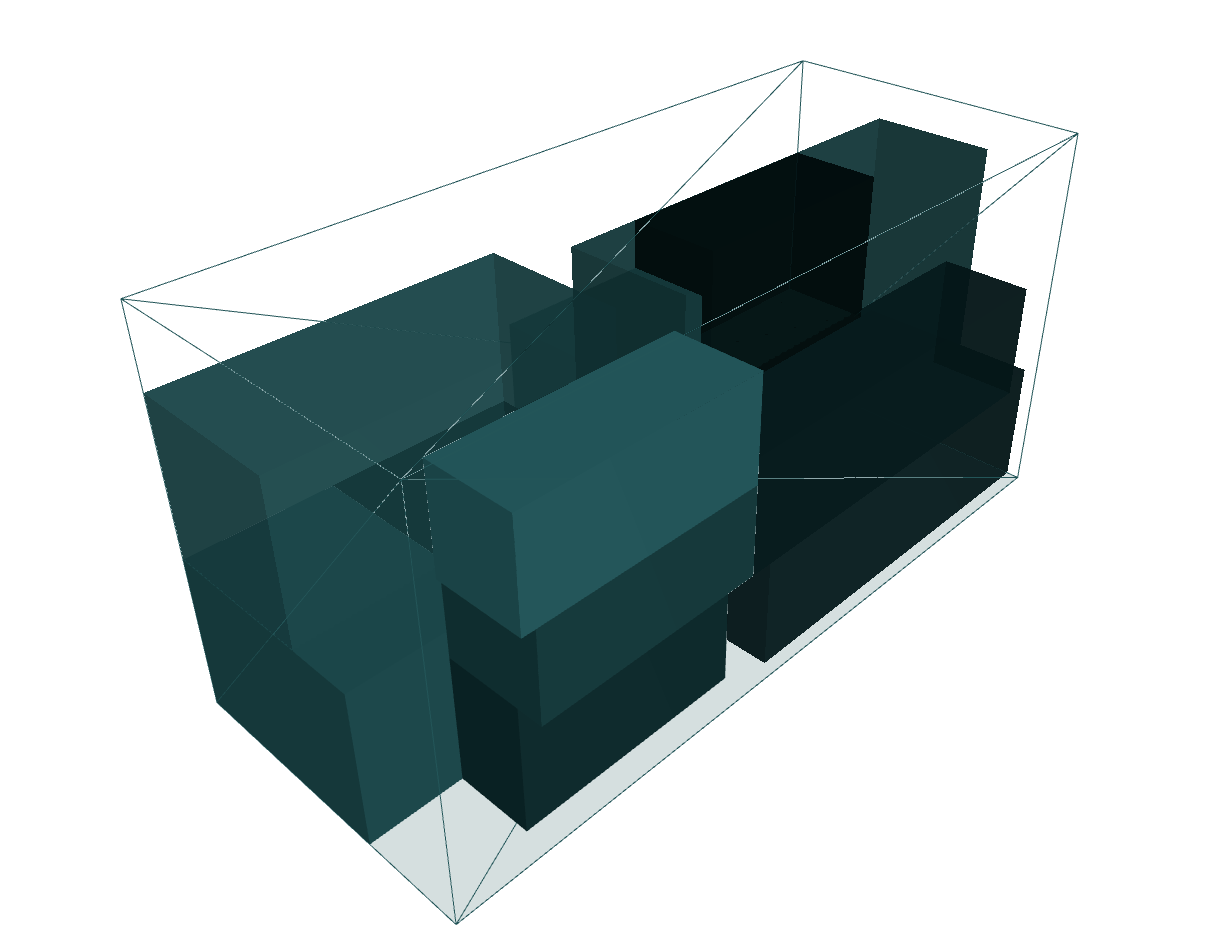
\includegraphics[width=7cm]{pictures/3l_cvrp_example.png}
    \caption{Visualized 3D packing with packing constraints\footnotemark}.
    \footnotetext{Visualization from \cite{tamke_branch-and-cut_2024}}
    \label{fig:solution-visualization}
\end{figure}

According to \cite{bischoff_issues_1995}, the mere placement of items is insufficient
if practical requirements are not fulfilled. Building on this insight,
\cite{bortfeldt_constraints_2013} systematically categorized all constraints relevant
to the \gls{CLP} into five groups. They also distinguish between hard and soft constraints,
where hard constraints must be strictly satisfied, while soft constraints may be violated
to some extent, depending on the implementation context.
It should also be noted that, by referring to the standard problems of \gls{CaP},
certain assumptions are implicitly adopted. For instance, in line with common
practice in the literature only orthogonal placements are allowed, so box surfaces must be
aligned parallel to the container floor and walls \footcite[cf.][p.2]{bortfeldt_constraints_2013}

\subsubsection{Container related constraints}
These constraints summarize all physical barriers of the container, including
the accumulated \textbf{weight} and \textbf{volume} of the cargo. The distribution of the weight
(\textbf{load balance}) plays also an important role for safety reasons, as the
cargo must not move during the transport and the container must not tip over.
In the special case of trucks, uneven axle weight distribution can cause severe
crash consequences and need to be avoided \footcite[cf.][p.849-850]{krebs_advanced_2021}.

\subsubsection{Item related constraints}
Item related constraints define the properties of the item, which are relevant
for the packing. When the container capacity is limited (\textit{output maximization}),
the \textbf{loading priority} constraint can define the priority among possible
item candidates. The orientation constraint limits how the item
can be rotated: it can either rotate only around the z-axis or be completely
free to rotate in all directions, with no partial flexibility in between.
When three dimesional packing is considered, the \textbf{stacking} constraint
is relevant for defining which items can be packed on top of each other. \cite{gendreau_tabu_2006}
differentiates between \textit{fragile} and \textit{non-fragile} items, stating
that non-fragile items can only be stacked on non-fragile items, Figure \ref{fig:stacking_comparison} showcases
this definition. A more sophisticated approach is the calculation  of the
\textit{load-bearing strength} of each box, stating how much pressure the box
can tolerate \footcite[cf.][p.847-848]{krebs_advanced_2021}.

\begin{figure}[htbp]
    \centering
    % First TikZ picture
    \begin{subfigure}[b]{0.45\textwidth}
        \centering
        \begin{tikzpicture}
            % Draw the container
            \draw[thick] (0,0) rectangle (5,3);

            % Draw the three items inside
            \draw[fill=blue!20] (3,0) rectangle (5,0.75);
            \node at (4, 0.5) {};

            \draw[fill=green!20] (3,0.75) rectangle (5,1.5);
            \node at (4, 1.125) {Fragile};

            \draw[fill=green!20] (3,1.5) rectangle (5, 2.25);
            \node at (4, 1.875) {Fragile};

        \end{tikzpicture}
        \caption{Feasible stacking of items}
    \end{subfigure}
    \hfill
    % Second TikZ picture
    \begin{subfigure}[b]{0.45\textwidth}
        \centering
        \begin{tikzpicture}
            \draw[thick] (0,0) rectangle (5,3);

            % Draw the three items inside
            \draw[fill=blue!20] (3,0) rectangle (5,0.75);
            \node at (4, 0.5) {};

            \draw[fill=green!20] (3,0.75) rectangle (5,1.5);
            \node at (4, 1.125) {Fragile};

            \draw[fill=blue!20] (3,1.5) rectangle (5, 2.25);
            \node at (4, 1.875) {};
        \end{tikzpicture}
        \caption{Infeasible stacking of items}
    \end{subfigure}
    \caption[Visualization fragile stacking]{Comparison fragile stacking \footnotemark}
    \footnotetext{Own figure}
    \label{fig:stacking_comparison}
\end{figure}


\subsubsection{Cargo-Related Constraints}
In contrast to item-related constraints, cargo-related constraints apply to
the entire cargo or to specific subsets of it. The \textbf{complete-shipment constraint}
requires that all items within a shipment must either be loaded into the same
container or be left behind entirely. This constraint is especially important
when container capacity is limited (\textit{output maximization}) and items
cannot be split.The \textbf{allocation constraint} serves a similar purpose.
It includes the \textbf{connectivity constraint}, which mandates that
certain items must be loaded into the same container, and the
\textbf{separation constraint}, which requires specific items to
be distributed across different containers. For example, kitchen
shipments—comprising multiple packages-should be delivered together
to enable efficient installation. Conversely, items such as perfume and fresh
vegetables should be shipped separately due to incompatibility.

\subsubsection{Positioning constraints}

Positioning constraints in container loading determine where items are placed,
either in absolute or relative terms, and can be modeled as hard or soft
constraints. It can be differentiated in seveeral groups. The
\textbf{absolute positioning constraints} specify that certain items
must (or must not) be placed in specific areas of the container. These are
typically based on item characteristics such as size, weight, or
content (e.g., bulky or hazardous items placed near the container door for accessibility).
\textbf{Relative positioning constraints} govern how items are arranged in
relation to each other. Either close to each other as \textit{group} or
\textit{separate} from each other. This differentiation is similar to the
\textit{allocation constraint} of the cargo-related constraints, but considers
only one container. The \textbf{multi-drop constraints} combine
absolute and relative positioning requirements when items are destined for
different deliverym locations. These constraints aim to minimize reloading
efforts by grouping items by delivery destination, by arranging item groups
in accordance with the delivery sequence and/or by applying a
\textit{\gls{LIFO}} or \textit{sequential loading policy}
to ensure efficient unloading without moving unrelated items. These
types of positioning constraints are widely discussed in the iterature due
to their practical relevance in real-world logistics operations.

\subsubsection{Load-related constraints}

The \textbf{stability constraint} is defined as one of the most critical constrains
in the \gls{CLP}, as it directly impacts
the safety of both the cargo and the personnel involved. First, a distinction
must be made between \textit{horizontal} and \textit{vertical} stability.
Horizontal stability is achieved when items are securely connected to the
container walls or to other items, preventing lateral movement. Vertical
stability, on the other hand, is defined in various ways throughout the
literature. One common approach evaluates the supporting area — the portion
of an item's base that rests on the surface below. Stability is often
considered sufficient if the support area covers between 70\% and 100\% of the base
of the item stacked on top. However, this can still cause unstable
configurations (see Figure~\ref{fig:vertical_stability_comparison}). To address this,
a more robust definition of vertical stability involves the
\textit{center of balance} of the upper item. According to this definition,
vertical stability is ensured only if the center of balance of the item on top
lies within the supporting area of the item below. It is also essential to
ensure that the load remains stable even after parts of the cargo have been
unloaded. In addition, \textbf{complexity constraints} refer to specialized
requirements that extend beyond standard packing rules. These include,
for example, compatibility with automated or robot-assisted packing systems.

\begin{figure}[htbp]
    \centering
    % First TikZ picture
    \begin{subfigure}[b]{0.45\textwidth}
        \centering
        \begin{tikzpicture}
            % Draw the container
            \draw[thick] (0,0) rectangle (5,3);

            % Draw the three items inside
            \draw[fill=blue!20] (3,0) rectangle (5,0.5);
            \draw[fill=blue!20] (2.5,0.5) rectangle (4.5,1);
            \draw[fill=blue!20] (2,1) rectangle (4, 1.5);
            \draw[fill=blue!20] (1.5,1.5) rectangle (3.5, 2);
            \draw[fill=blue!20] (1,2) rectangle (3, 2.5);
            \draw[fill=blue!20] (0.5,2.5) rectangle (2.5, 3);
            %\node at (4, 1.875) {Fragile};
            \draw[thick,dashed] (2.75,0) -- (2.75,3);  % <---
            \node[anchor = west,align=center] at (2.9,2.5) {\small Center of \\  balance};

        \end{tikzpicture}
        \caption[align = center]{Feasible stacking with 75\% support area; infeasible due to unstable center}
    \end{subfigure}
    \hfill
    % Second TikZ picture
    \begin{subfigure}[b]{0.45\textwidth}
        \centering
        \begin{tikzpicture}
            % Draw the container
            \draw[thick] (0,0) rectangle (5,3);

            % Draw the three items inside
            \draw[fill=green!20] (3,0) rectangle (5,0.5);
            \draw[fill=green!20] (1,0) rectangle (3,0.5);

            \draw[fill=green!20] (2.5,0.5) rectangle (4.5,1);
            \draw[fill=green!20] (0.5,0.5) rectangle (2.5,1);

            \draw[fill=green!20] (1.5,1) rectangle (3.5, 1.5);
            \draw[fill=green!20] (1.5,1.5) rectangle (3.5, 2);
            \draw[fill=green!20] (2,2) rectangle (3, 2.5);

            \draw[thick,dashed] (2.5,0) -- (2.5,3);  % <---
            \node[anchor = west,align=center] at (2.9,2.5) {\small Center of \\  balance};
        \end{tikzpicture}
        \caption[align = center]{Feasible stacking regarding 75\% support area and stable center}
    \end{subfigure}
    \caption[Visualization vertical stability]{Comparison vertical stability (side view) \footnotemark}
    \footnotetext{Own figures based on \cite[p.845]{krebs_advanced_2021}}
    \label{fig:vertical_stability_comparison}
\end{figure}


\begin{comment}
Eventuelle Tabelle!, die darstelt welche constraints in der Literatur zu finden
und welche nicht
\end{comment}
% Main Part
\chapter{Zweites Kapitel}

\section{Erster Abschnitt des zweiten Kapitels}

Text Text Text Text Text Text Text Text Text Text Text Text Text Text Text Text Text Text Text Text Text Text Text Text Text Text Text Text Text Text Text Text Text Text Text Text Text Text Text Text Text Text Text Text Text Text Text Text Text Text Text Text Text Text Text Text Text Text Text Text Text Text Text Text Text Text Text Text Text Text Text Text Text Text Text Text Text Text Text Text Text Text Text Text Text Text Text Text Text Text Text Text Text Text Text Text Text Text Text Text Text Text Text. Wie im Algorithmus~\ref{alg:euclid} dargestellt\dots

\begin{algorithm}[htb]
	\caption{Euclid's Algorithmus}\label{alg:euclid}
	\begin{algorithmic}[1]
		\Procedure{Euclid}{$a,b$}\Comment{Der größte gemeinsame Teiler (ggT) von $a$ und $b$}
			\State $r \gets a \bmod b$
			\While{$r\not=0$}\Comment{Das Ergebnis liegt vor wenn $r=0$}
				\State $a \gets b$
				\State $b \gets r$
				\State $r \gets a \bmod b$
			\EndWhile
			\State \textbf{return} $b$ \Comment{Der ggT ist $b$}
		\EndProcedure
	\end{algorithmic}
\end{algorithm}

Text Text Text Text Text Text Text Text Text Text Text Text Text Text Text Text Text Text Text Text Text Text Text Text Text Text Text Text Text Text Text Text Text Text Text Text Text Text Text Text Text Text Text Text Text Text Text Text Text Text Text Text Text Text Text Text Text Text Text Text Text Text Text Text Text Text Text Text Text Text Text Text Text Text Text Text Text Text Text Text Text Text Text Text Text Text Text Text Text Text Text Text Text Text Text Text Text Text Text Text Text Text Text.

\section{Zweiter Abschnitt des zweiten Kapitels}

Text Text Text Text Text Text Text Text Text Text Text Text Text Text Text Text Text Text Text Text Text Text Text Text Text Text Text Text Text Text Text Text Text Text Text Text Text Text Text Text Text Text Text Text Text Text Text Text Text Text Text Text Text Text Text Text Text Text Text Text Text Text Text Text Text Text Text Text Text Text Text Text Text Text Text Text Text Text Text Text Text Text Text Text Text Text Text Text Text Text Text Text Text Text Text Text Text Text Text Text Text Text Text.

\section{Dritter Abschnitt des dritten Kapitels}

Text Text Text Text Text Text Text Text Text Text Text Text Text Text Text Text Text Text Text Text Text Text Text Text Text Text Text Text Text Text Text Text Text Text Text Text Text Text Text Text Text Text Text Text Text Text Text Text Text Text Text Text Text Text Text Text Text Text Text Text Text Text Text Text Text Text Text Text Text Text Text Text Text Text Text Text Text Text Text Text Text Text Text Text Text Text Text Text Text Text Text Text Text Text Text Text Text Text Text Text Text Text Text.

Geht das jetzt? Ja :D 


%####################### Appendix #########################
%%############################# Anhang #################################
%\appendix
%\chapter{Mathematischer Anhang}
%\chapter{Programmcodes}

\clearpage
%####################### Literaturverzeichnis #########################
\addcontentsline{toc}{chapter}{\bibname}
\printbibliography
%####################### Selbständigkeitserklärung ####################

\newConfirmationEnglish{Dresden}

%####################### Platzhalter - Abkürzungsverzeichnis muss erstellt werden####################

\printacronyms[style=bwlimsuper]

%####################### End of Document ####################
\end{document}